\documentclass[aspectratio=169,11pt]{beamer}
\usepackage{beamerucad}
\usepackage{listings}
\definecolor{ckw}{HTML}{2563AB}\definecolor{cst}{HTML}{2E8B57}\definecolor{ccm}{HTML}{8A8F98}
\lstdefinestyle{py}{language=Python,basicstyle=\ttfamily\footnotesize,
 keywordstyle=\color{ckw}\bfseries,stringstyle=\color{cst},commentstyle=\color{ccm}\itshape,
 showstringspaces=false,columns=fullflexible,keepspaces=true,
 backgroundcolor=\color{ucadband!8},frame=leftline,framerule=2.5pt,rulecolor=\color{ucadband},
 xleftmargin=8pt,aboveskip=3pt,belowskip=1pt,basewidth=0.5em}
\lstset{style=py}
\title{Introduction au ML — Séance 8}
\subtitle{La force du nombre : les méthodes d'ensemble}
\author{Dr. El Hadji Bassirou TOURÉ}
\institute{Département de Mathématiques et Informatique\\ Faculté des Sciences et Techniques\\ Université Cheikh Anta Diop de Dakar}
\date{}
\setucadfoot{Introduction au ML --- Séance 8 \quad\textbullet\quad Dr. El Hadji Bassirou TOURÉ --- DMI/FST/UCAD}
\graphicspath{{figs/}}
\begin{document}

\begin{frame}[plain,noframenumbering]\titlepage\end{frame}

\begin{frame}{Objectifs de la séance}
\begin{ucaddef}[Contenu]
{\small La Séance 7 a réglé un arbre du mieux possible : bien dosé, il atteignait AUC $0{,}73$ sur le paludisme — puis butait. Cette séance dépasse ce plafond non pas en perfectionnant \emph{un} modèle, mais en en combinant \emph{beaucoup}, selon deux philosophies opposées.}
\end{ucaddef}
\begin{itemize}\small
  \item La \textbf{sagesse de la foule} : pourquoi, et à quelle condition, agréger des modèles médiocres bat un expert unique.
  \item Le \textbf{bagging} : le rééchantillonnage \emph{bootstrap}, l'agrégation, et l'évaluation \emph{out-of-bag} gratuite.
  \item La \textbf{forêt aléatoire} : décorréler les arbres (et pourquoi cela compte \emph{quantitativement}), l'importance des variables et son piège.
  \item Le \textbf{boosting} : des arbres séquentiels qui corrigent leurs erreurs ; le gradient boosting comme descente de gradient.
  \item \textbf{Bagging contre boosting}, et la leçon centrale : le modèle le plus puissant n'est pas toujours le meilleur.
\end{itemize}
\end{frame}

% #####################################################################
\section{Le plafond de l'arbre unique}

\begin{frame}{Le dilemme de l'arbre seul}
\begin{ucadfront}[Souple ou stable : il faut choisir]
{\small Un arbre profond mémorise l'entraînement — \textbf{variance élevée} : déplacez quelques patients, et l'arbre change du tout au tout. Un arbre bridé généralise mais manque de finesse — \textbf{biais élevé}. La validation croisée (Séance 7) trouvait le meilleur compromis, mais ce compromis est un \emph{plafond} : un seul arbre ne peut être à la fois souple et stable.}
\end{ucadfront}
{\small Rappel chiffré de la Séance 7, sur la durée d'hospitalisation : l'arbre de profondeur $10$ obtenait $R^2 = 0{,}726$ en entraînement mais $0{,}461$ en test — l'écart signe la variance. Le bridant à la profondeur $6$, on stabilisait à $R^2 \approx 0{,}55$, sans jamais aller plus haut.}
\end{frame}

\begin{frame}{L'idée de la séance : contourner le dilemme}
\begin{ucaddef}[L'idée en une phrase]
{\small Plutôt que de chercher \emph{l'}arbre parfaitement dosé, on laisse chaque arbre être imparfait — puis on en combine un grand nombre, de sorte que leurs défauts se compensent.}
\end{ucaddef}
{\small Deux façons de combiner, qui structurent toute la séance :}
\begin{itemize}\small
  \item laisser les arbres \textbf{instables} (profonds, à variance élevée) et \textbf{moyenner} pour effacer la variance — c'est le \emph{bagging} et les \emph{forêts} ;
  \item prendre des arbres \textbf{trop simples} (à biais élevé) et les \textbf{enchaîner} pour effacer le biais — c'est le \emph{boosting}.
\end{itemize}
{\small Réduire la variance, ou réduire le biais : deux familles, deux mécaniques, qu'il faut comprendre séparément avant de les opposer.}
\end{frame}

% #####################################################################
\section{La sagesse de la foule}

\begin{frame}{L'idée : un jury vaut mieux qu'un juge}
\begin{ucadfront}[Analogie]
{\small Un jury de quartier juge une affaire. Chaque juré pris isolément se trompe souvent — disons une fois sur trois. Mais si leurs erreurs sont \emph{indépendantes} (ils ne se copient pas), la \textbf{majorité} se trompe bien plus rarement que chacun : les fautes des uns sont noyées par les votes corrects des autres. Un collège de votants médiocres mais variés surpasse n'importe lequel d'entre eux.}
\end{ucadfront}
\begin{ucaddef}[L'idée en une phrase]
{\small Agréger les prédictions de nombreux modèles \textbf{décorrélés} fait tomber l'erreur de l'ensemble en dessous de l'erreur de chaque membre — à la stricte condition que leurs erreurs ne soient pas les mêmes.}
\end{ucaddef}
\end{frame}

\begin{frame}{La foule, formellement}
\begin{ucaddef}[Définition]
{\small Pour $M$ votants indépendants ayant chacun raison avec probabilité $p > 0{,}5$, la probabilité que la \emph{majorité} ait raison suit une loi binomiale, et croît vers $1$ avec $M$.}
\end{ucaddef}
\ucadformula{P(\text{majorité correcte}) \;=\; \sum_{k > M/2} \binom{M}{k}\, p^k (1-p)^{M-k}}
{\small Pour $p > 0{,}5$, cette somme tend vers $1$ quand $M$ grandit (théorème du jury de Condorcet, 1785). La condition $p > 0{,}5$ est indispensable : si chaque votant fait \emph{pire} que le hasard, la majorité empire elle aussi. Et tout repose sur l'\textbf{indépendance} — la formule binomiale n'est valable que si les erreurs ne sont pas corrélées.}
\end{frame}

\begin{frame}{Exemple — la foule en chiffres}
\begin{columns}[c]
\column{0.45\linewidth}
{\small Des jurés indépendants, chacun correct à $65\,\%$, décision à la majorité :
\begin{center}\renewcommand{\arraystretch}{1.15}
\begin{tabular}{c|c}
nombre de jurés & majorité correcte\\\hline
$1$ & $0{,}650$\\
$3$ & $0{,}718$\\
$11$ & $0{,}851$\\
$51$ & $0{,}986$\\
\end{tabular}\end{center}}
\column{0.53\linewidth}
\centering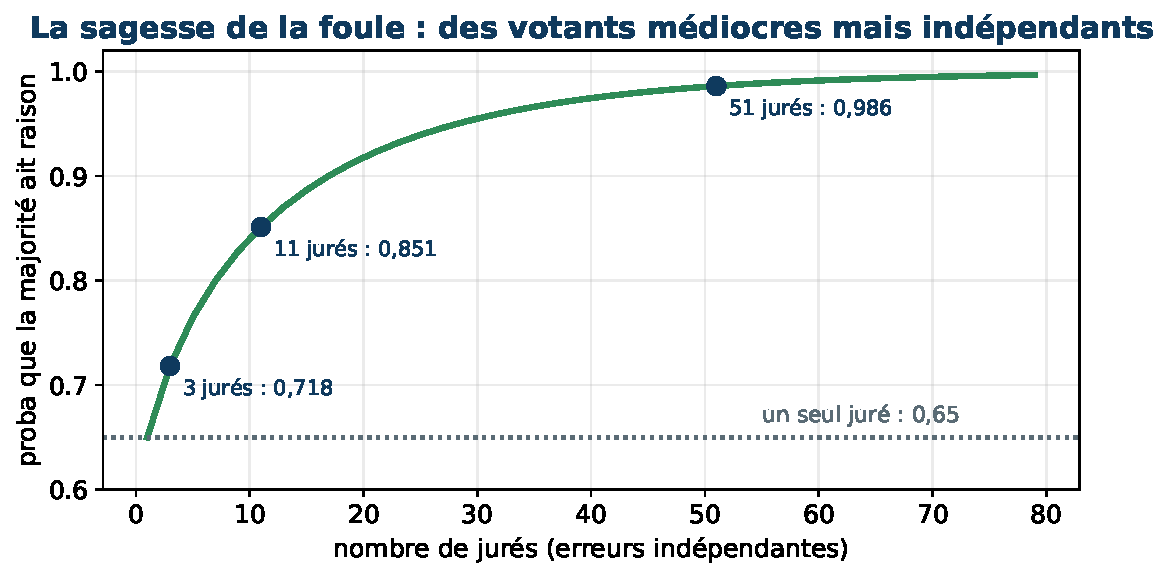
\includegraphics[width=\linewidth]{f8_foule}
\end{columns}
\vspace{2pt}

{\small Onze votants à $65\,\%$ atteignent $85\,\%$ ; cinquante et un, près de $99\,\%$. \textbf{Mais} l'indépendance est tout : cinquante et un jurés qui copient le même se trompent encore $35\,\%$ du temps. Tout l'art du métier sera de fabriquer des arbres qui \emph{ne se ressemblent pas}.}
\end{frame}

\begin{frame}{Le lien avec biais et variance}
\begin{ucaddef}[Pourquoi moyenner aide — et ce que ça ne corrige pas]
{\small Moyenner plusieurs modèles ne change pas leur \emph{biais} commun : si tous se trompent dans le même sens, la moyenne aussi. En revanche, cela réduit leur \emph{variance} — les écarts individuels dus au hasard du tirage se compensent. C'est exactement le profil d'un arbre profond : beaucoup de variance, peu de biais.}
\end{ucaddef}
{\small De là, les deux stratégies de la séance, désormais nommées précisément : \textbf{(1)} prendre des modèles à \emph{variance} élevée et la faire tomber en moyennant — le bagging et les forêts ; \textbf{(2)} prendre des modèles à \emph{biais} élevé et le réduire en les enchaînant — le boosting. La prochaine section quantifie exactement de combien moyenner réduit la variance, et pourquoi la décorrélation y est décisive.}
\end{frame}

\begin{frame}{Exercice — la foule est-elle toujours sage ?}
\begin{ucadrec}[Énoncé]
{\small (a) Onze médecins indépendants diagnostiquent juste à $70\,\%$ ; la majorité fait-elle mieux ou moins bien que chacun ? (b) Onze médecins qui se concertent et rendent tous le \emph{même} avis (corrélation parfaite) : que vaut leur « majorité » ? (c) Onze médecins indépendants justes à seulement $40\,\%$ : la foule aide-t-elle ?}
\end{ucadrec}
\pause
\begin{ucadex}[Correction]
{\small \textbf{(a)} Mieux : avec $p = 0{,}70 > 0{,}5$ et l'indépendance, la majorité dépasse $0{,}70$ (et grimpe vers $1$ avec le nombre). \textbf{(b)} Exactement $0{,}70$ — onze avis identiques valent un seul avis ; la corrélation parfaite annule tout le bénéfice de la foule. \textbf{(c)} Non, elle \emph{aggrave} : $p = 0{,}40 < 0{,}5$, donc la majorité fait \emph{pire} que $40\,\%$ — une foule de votants sous le hasard converge vers l'erreur. Conditions vitales : $p > 0{,}5$ \emph{et} indépendance.}
\end{ucadex}
\end{frame}

% #####################################################################
\section{Le bagging}

\begin{frame}{L'idée : varier les données pour varier les arbres}
\begin{ucaddef}[L'idée en une phrase]
{\small Pour fabriquer des arbres différents à partir d'un \emph{seul} jeu de données, on entraîne chacun sur un \textbf{échantillon bootstrap} — un tirage avec remise de même taille — puis on agrège : vote majoritaire en classification, moyenne en régression. C'est le \textbf{bagging} (\emph{bootstrap aggregating}).}
\end{ucaddef}
{\small Chaque arbre voit une version légèrement déformée des données : certains patients en double, d'autres absents. Les arbres diffèrent donc, leurs erreurs se décorrèlent \emph{un peu}, et la moyenne gagne en stabilité. Reste à comprendre ce qu'est précisément ce tirage, et combien il laisse de patients de côté.}
\end{frame}

\begin{frame}{Le mécanisme — le bootstrap, à la main}
\begin{ucadex}[Un tirage avec remise sur six patients]
{\small Six patients numérotés $1$ à $6$. Un échantillon bootstrap tire $6$ fois \emph{avec remise} — un même patient peut sortir plusieurs fois, un autre pas du tout :
\[ \text{tirage} : \{2,\ 3,\ 4,\ 5,\ 5,\ 6\} \;\Rightarrow\; \text{vus} : \{2,3,4,5,6\}, \quad \text{absent} : \{1\}. \]
Le patient $5$ compte double (il pèsera plus dans cet arbre) ; le patient $1$ n'a pas servi — il est \textbf{out-of-bag} (OOB) pour cet arbre. Un autre arbre tirera un autre échantillon, laissera d'autres patients de côté : c'est cette diversité qui décorrèle les arbres.}
\end{ucadex}
{\small Sur un grand jeu, la proportion de patients \emph{vus} se stabilise à une valeur remarquable — que le calcul suivant établit.}
\end{frame}

\begin{frame}{Pourquoi 63 \% ? le calcul détaillé}
\begin{ucaddef}[La limite $1 - 1/e$]
{\small À chaque tirage, un patient donné a une chance $\tfrac{1}{n}$ d'être choisi, donc $1 - \tfrac{1}{n}$ de \emph{ne pas} l'être. Les $n$ tirages étant indépendants, la probabilité qu'il soit absent des $n$ tirages est le produit.}
\end{ucaddef}
\ucadformula{P(\text{absent}) = \Big(1 - \tfrac{1}{n}\Big)^{n} \xrightarrow[n \to \infty]{} \frac{1}{e} \approx 0{,}368}
{\small (Rappel : $\big(1 + \tfrac{x}{n}\big)^n \to e^{x}$ ; ici $x = -1$, d'où $e^{-1}$.) Donc un patient a $\approx 37\,\%$ de chances d'être out-of-bag, et $\approx \mathbf{63\,\%}$ de figurer dans l'échantillon. Vérification : $n = 6 \to 0{,}335$ ; $n = 100 \to 0{,}366$ ; $n = 10\,000 \to 0{,}368$. La convergence est rapide.}
\centering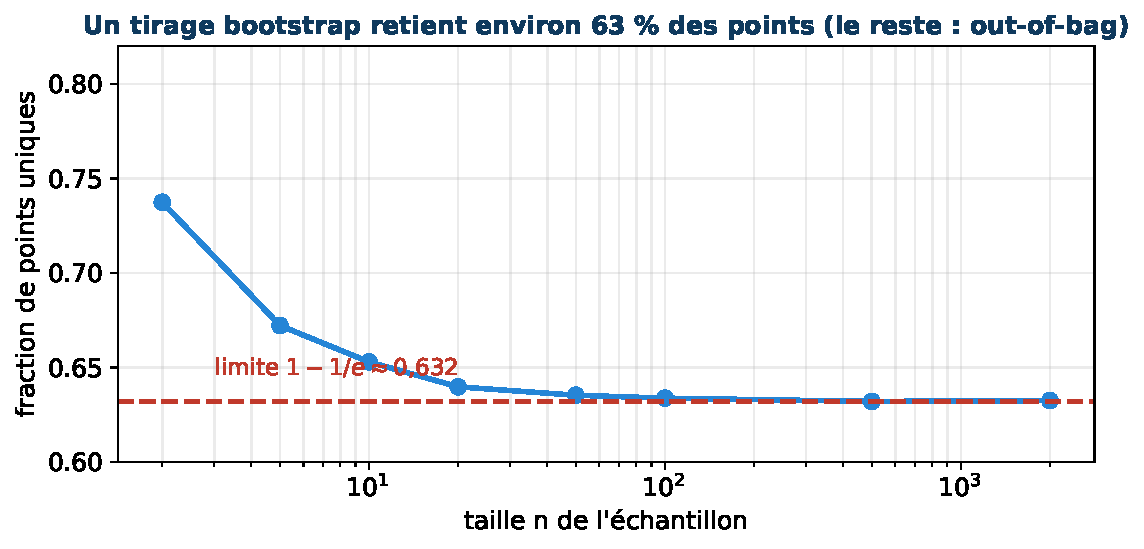
\includegraphics[width=0.38\linewidth]{f8_bootstrap}
\end{frame}

\begin{frame}{Le schéma du bagging}
\centering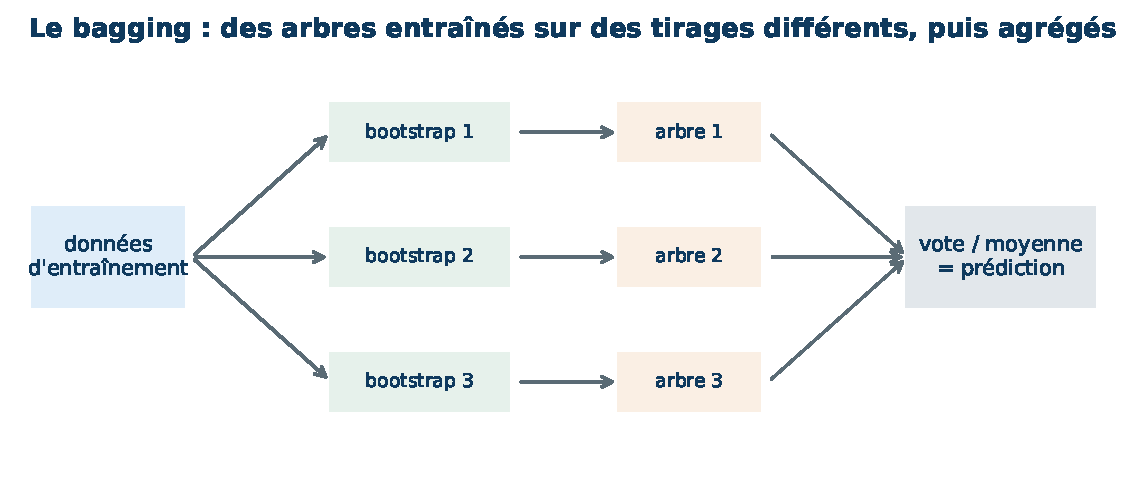
\includegraphics[width=0.80\linewidth]{f8_bagging}
\vspace{2pt}

{\small Un seul jeu de données engendre plusieurs échantillons bootstrap ; un arbre par échantillon, entraîné indépendamment ; les prédictions sont agrégées en une seule (moyenne ou vote). Chaque arbre est individuellement instable — mais leurs instabilités se compensent à l'agrégation. Comme les arbres ne dépendent pas les uns des autres, on peut les entraîner \emph{en parallèle}.}
\end{frame}

\begin{frame}{Le bagging, formellement}
\begin{ucaddef}[Définition]
{\small Soit $B$ échantillons bootstrap, et $\hat f_b$ l'arbre entraîné sur le $b$-ième. La prédiction du bagging agrège les $B$ arbres : par moyenne des probabilités (classification, ou régression), ou par vote majoritaire des classes.}
\end{ucaddef}
\ucadformula{\hat f_{\text{bag}}(x) \;=\; \frac{1}{B}\sum_{b=1}^{B} \hat f_b(x)}
{\small Les arbres baggés sont délibérément \emph{profonds} (non élagués) : leur biais est faible, et le bagging se charge d'écraser leur variance. C'est l'inverse du réflexe « bridons l'arbre » de la Séance 7 — ici, on \emph{veut} des arbres instables, car on dispose du moyen de les stabiliser collectivement.}
\end{frame}

\begin{frame}{L'évaluation out-of-bag : une validation gratuite}
\begin{ucaddef}[L'idée en une phrase]
{\small Puisque chaque patient est OOB pour environ un tiers des arbres, on peut le faire prédire \emph{par ces arbres-là seulement} — qui ne l'ont jamais vu. En agrégeant ces prédictions OOB sur tous les patients, on obtient une estimation de performance \textbf{sans réserver de jeu de validation}.}
\end{ucaddef}
{\small Le mécanisme reproduit exactement l'esprit de la validation croisée (Séance 7) — juger chaque donnée par des modèles qui l'ignorent — mais il est offert par le bagging sans calcul supplémentaire : les arbres qui n'ont pas vu un patient existent déjà, il suffit de les interroger. C'est un avantage propre aux méthodes baggées.}
\end{frame}

\begin{frame}{Exemple — l'out-of-bag sur le paludisme}
\begin{ucadex}[Un score gratuit]
{\small Un bagging de $100$ arbres sur le paludisme affiche un \textbf{score OOB} de $0{,}869$ (accuracy), calculé sans toucher au test : chaque patient d'entraînement a été prédit par les $\approx 37$ arbres qui ne l'avaient pas dans leur échantillon. C'est un diagnostic immédiat de la qualité de l'ensemble, disponible à la fin du \texttt{fit}.}
\end{ucadex}
{\small Deux nuances. L'OOB est une accuracy : sur cette classe rare ($11{,}8\,\%$ de positifs), $0{,}869$ doit se lire \emph{en regard de la baseline} $0{,}882$ (Séance 6) — ce bagging ne la bat pas en accuracy, et il faudra le juger à l'AUC. Et le test reste \textbf{scellé} : l'OOB sert au développement, pas au verdict final.}
\end{frame}

\begin{frame}{Exercice — bootstrap et out-of-bag}
\begin{ucadrec}[Énoncé]
{\small Un échantillon bootstrap est tiré sur cinq patients $\{1,2,3,4,5\}$ ; le tirage donne $\{2,\ 2,\ 4,\ 5,\ 5\}$. (a) Quels patients sont vus, lesquels sont out-of-bag ? (b) Le patient $3$ peut-il servir à évaluer l'arbre entraîné sur ce tirage, et pourquoi ? (c) Sur un très grand jeu, quelle fraction de patients un échantillon bootstrap laisse-t-il en moyenne de côté ?}
\end{ucadrec}
\pause
\begin{ucadex}[Correction]
{\small \textbf{(a)} Vus : $\{2, 4, 5\}$ (le $2$ et le $5$ comptent double) ; out-of-bag : $\{1, 3\}$. \textbf{(b)} Oui — le patient $3$ n'a pas servi à entraîner cet arbre, il en est OOB ; le faire prédire par cet arbre est une évaluation honnête, car l'arbre ne l'a jamais mémorisé. \textbf{(c)} Environ $1/e \approx \mathbf{37\,\%}$ sont laissés de côté (et $\approx 63\,\%$ retenus) — la limite de $\big(1 - 1/n\big)^n$.}
\end{ucadex}
\end{frame}

% #####################################################################
\section{La forêt aléatoire}

\begin{frame}{Pourquoi le bagging ne suffit pas toujours}
\begin{ucadpiege}[Des arbres baggés peuvent rester semblables]
{\small Si une variable est très prédictive, \emph{tous} les arbres baggés la choisissent en haut de leur structure — ils se ressemblent malgré le bootstrap, et leurs erreurs restent fortement corrélées. Or moyenner des modèles corrélés ne réduit presque pas la variance : le bénéfice de la foule s'effondre quand les votants se ressemblent.}
\end{ucadpiege}
{\small Pour mesurer l'enjeu, il faut quantifier exactement comment la \emph{corrélation} entre arbres limite la réduction de variance — c'est l'objet de la formule suivante, et elle justifiera à elle seule l'ingrédient des forêts.}
\end{frame}

\begin{frame}{Le cœur quantitatif : la variance d'une moyenne corrélée}
\begin{ucaddef}[Définition]
{\small La variance de la moyenne de $B$ modèles, chacun de variance $\sigma^2$ et deux à deux corrélés au coefficient $\rho$, n'est \emph{pas} $\sigma^2/B$ : un terme irréductible subsiste, gouverné par $\rho$.}
\end{ucaddef}
\ucadformula{\operatorname{Var}\!\Big(\tfrac{1}{B}\textstyle\sum_b \hat f_b\Big) \;=\; \rho\,\sigma^2 \;+\; \frac{1-\rho}{B}\,\sigma^2 \;\xrightarrow[B \to \infty]{}\; \rho\,\sigma^2}
{\small Lecture décisive : ajouter des arbres ($B \to \infty$) fait disparaître le second terme, mais \textbf{laisse $\rho\,\sigma^2$}. La variance de l'ensemble ne descend jamais sous la \emph{corrélation} entre arbres. Donc : pour gagner, il ne suffit pas d'ajouter des arbres — il faut \emph{baisser $\rho$}. C'est toute la raison d'être de la forêt aléatoire.}
\end{frame}

\begin{frame}{L'effet de la corrélation, en image}
\centering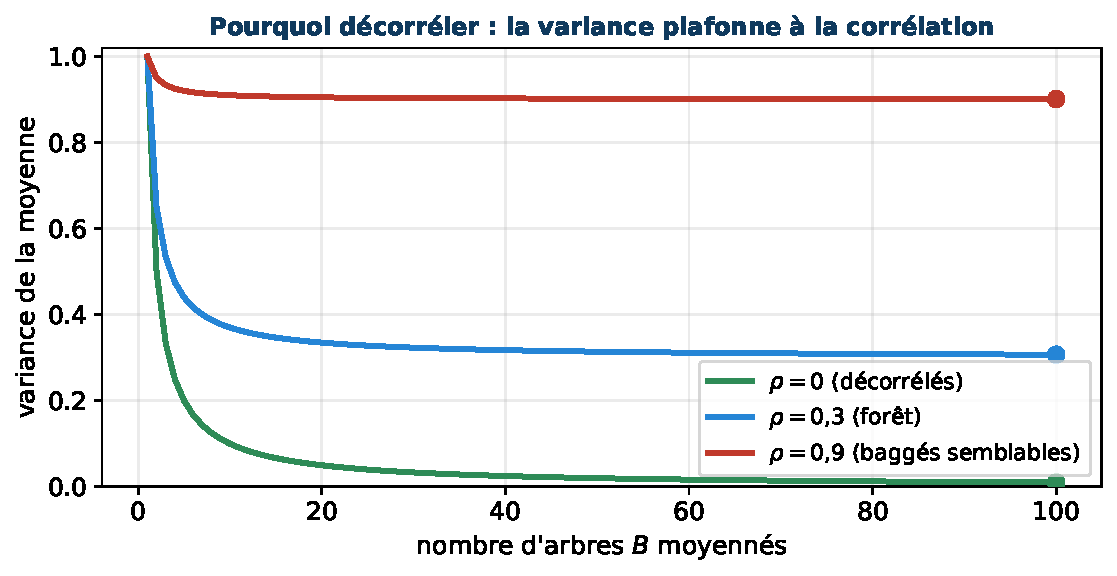
\includegraphics[width=0.60\linewidth]{f8_variance_moyenne}
\vspace{-2pt}

{\small À corrélation $\rho = 0{,}9$ (arbres baggés qui se ressemblent), cent arbres ne font tomber la variance que de $1{,}0$ à $0{,}90$ — presque rien. À $\rho = 0{,}3$ (arbres décorrélés), de $1{,}0$ à $0{,}31$. À $\rho = 0$ (idéal inatteignable), à $0{,}01$. Le message est sans appel : \textbf{la décorrélation, pas le nombre, est le vrai levier}. Reste à savoir comment décorréler — et la forêt a une idée simple.}
\end{frame}

\begin{frame}{L'idée de la forêt : décorréler à chaque coupure}
\begin{ucaddef}[L'idée en une phrase]
{\small La \textbf{forêt aléatoire} ajoute au bagging un second hasard : à \emph{chaque coupure} de chaque arbre, seules \texttt{max\_features} variables tirées au sort sont candidates. Aucun arbre ne peut alors s'appuyer systématiquement sur la même variable dominante — leur corrélation $\rho$ chute, et la moyenne devient bien plus efficace.}
\end{ucaddef}
{\small L'astuce est subtile : on \emph{dégrade volontairement} chaque arbre (en lui cachant des variables) pour \emph{améliorer} l'ensemble. Un arbre pris seul devient un peu moins bon ; mais comme les arbres se ressemblent moins, leur moyenne — la seule chose qui compte — gagne sur le tableau précédent.}
\end{frame}

\begin{frame}{La forêt aléatoire, formellement}
\begin{ucaddef}[Définition]
{\small Une forêt aléatoire est un bagging d'arbres profonds où chaque nœud ne choisit sa coupure que parmi \texttt{max\_features} variables tirées au hasard. La prédiction est la moyenne des probabilités des $B$ arbres ainsi décorrélés.}
\end{ucaddef}
\ucadformula{\hat p(x) \;=\; \frac{1}{B}\sum_{b=1}^{B} \hat p_b(x) \qquad (B = \texttt{n\_estimators},\ \text{coupures sur } \texttt{max\_features} \text{ variables})}
{\small Deux réglages principaux : \texttt{n\_estimators} (le nombre d'arbres) et \texttt{max\_features} (le degré de décorrélation). Le défaut de \texttt{max\_features} est $\sqrt{d}$ variables par coupure en classification — un point de départ éprouvé. Une variante, les \emph{extra-trees}, pousse le hasard plus loin en tirant aussi les \emph{seuils} au sort : encore plus de décorrélation, des arbres encore plus faibles.}
\end{frame}

\begin{frame}{Plus d'arbres : on gagne, puis on plafonne}
\centering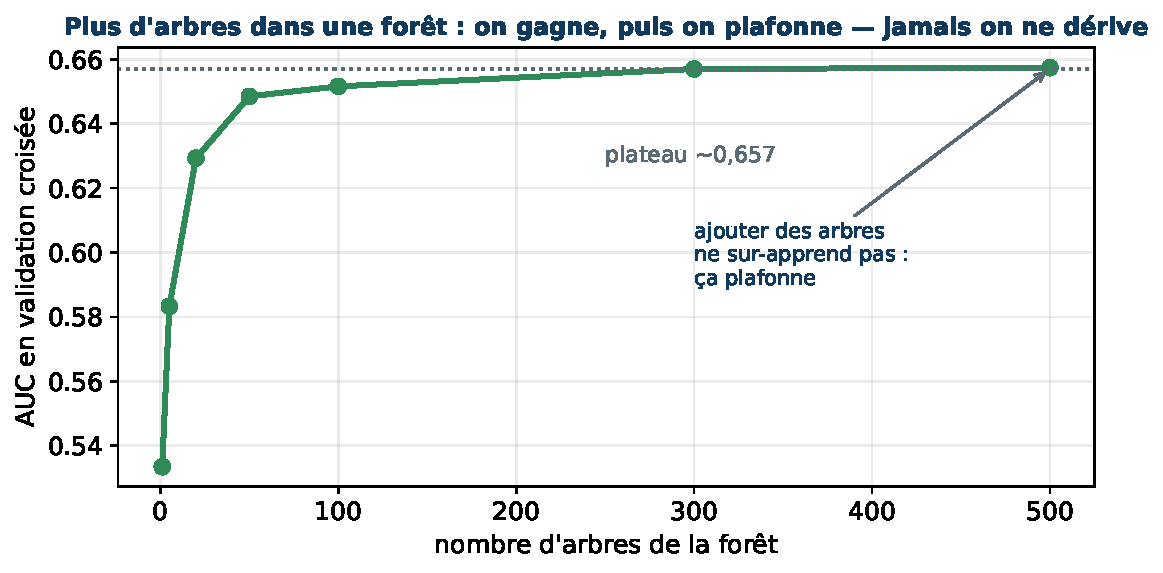
\includegraphics[width=0.58\linewidth]{f8_plateau}
\vspace{-2pt}

{\small AUC de validation croisée selon le nombre d'arbres : $1 \to 0{,}53$ ; $20 \to 0{,}63$ ; $100 \to 0{,}65$ ; $500 \to 0{,}66$. C'est la formule de variance en action : le terme $\tfrac{1-\rho}{B}\sigma^2$ s'éteint, on bute sur le plancher $\rho\,\sigma^2$. Propriété capitale qui en découle : ajouter des arbres à une forêt ne fait \textbf{jamais sur-apprendre} — la courbe monte puis plafonne. \texttt{n\_estimators} n'est donc pas à régler finement : on en met « assez » (quelques centaines), le surcoût est en temps de calcul, pas en qualité.}
\end{frame}

\begin{frame}{Le réglage de la décorrélation : max\_features}
\begin{ucaddef}[Le seul réglage vraiment sensible de la forêt]
{\small \texttt{max\_features} dose directement la corrélation $\rho$ : \emph{petit} $\Rightarrow$ arbres très décorrélés (mais chacun plus faible) ; \emph{grand} (toutes les variables) $\Rightarrow$ on retombe sur le bagging, $\rho$ élevé. C'est un compromis entre décorrélation et force individuelle.}
\end{ucaddef}
\begin{ucadex}[Sur le paludisme, AUC de validation croisée]
{\small \begin{center}\renewcommand{\arraystretch}{1.1}\begin{tabular}{l|ccccc}
\texttt{max\_features} & $1$ & $2$ & $3$ & $\sqrt{d}$ & toutes\\\hline
AUC CV & $0{,}659$ & $0{,}657$ & $0{,}649$ & $0{,}657$ & $0{,}647$\\
\end{tabular}\end{center}
La valeur la plus restrictive ($1$ variable par coupure) donne ici la meilleure AUC, et « toutes les variables » (le bagging pur) la plus faible — confirmation directe : sur ces données, plus on décorrèle, mieux c'est. L'écart reste modeste car le problème ne compte que $5$ variables.}
\end{ucadex}
\end{frame}

\begin{frame}{L'importance des variables}
\begin{ucaddef}[L'idée en une phrase]
{\small La forêt peut mesurer combien chaque variable a fait \emph{baisser l'impureté} (Gini, Séance 3), cumulé sur tous les nœuds qui l'utilisent et tous les arbres — donnant un classement de l'utilité apparente des variables.}
\end{ucaddef}
{\small C'est l'un des attraits majeurs des forêts : là où la logistique offrait des poids (Séance 6), la forêt offre un score d'importance par variable, applicable même quand les relations sont non linéaires. Séduisant — mais cette mesure recèle un piège sérieux, que le cas du paludisme va révéler crûment.}
\end{frame}

\begin{frame}{Le piège de l'importance par impureté}
\begin{columns}[c]
\column{0.42\linewidth}
\centering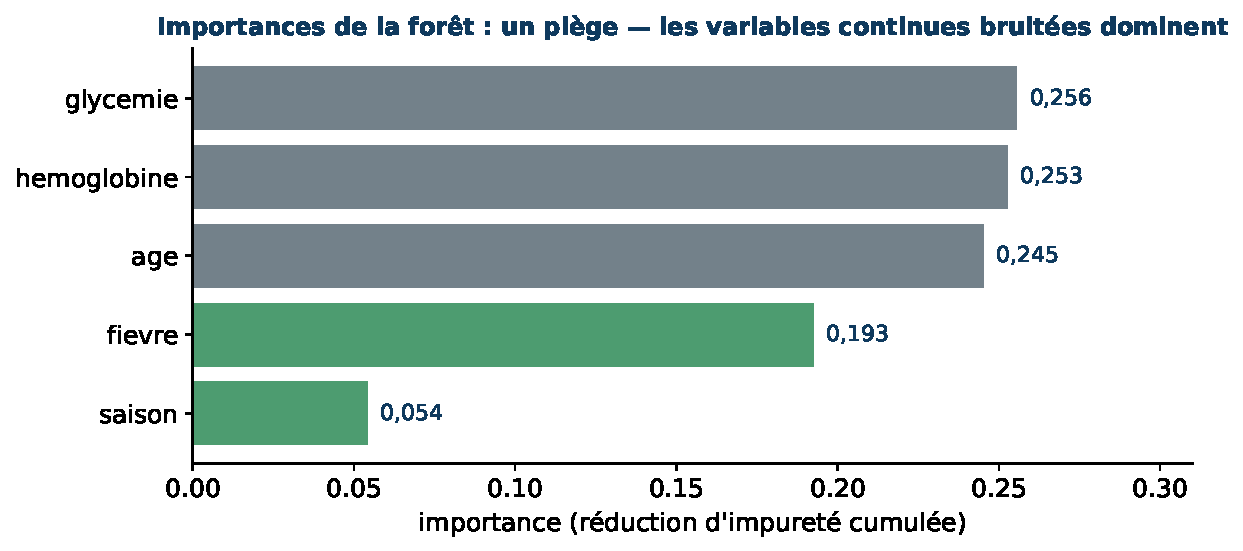
\includegraphics[width=\linewidth]{f8_importance}
\column{0.56\linewidth}
\begin{ucadpiege}[Lecture prudente]
{\small Sur le paludisme, glycémie, hémoglobine et âge ressortent « importantes » — alors que, \emph{par construction des données}, la maladie ne dépend que de la \textbf{saison} et de la \textbf{fièvre}. Pourquoi cette trahison ? Ces variables \textbf{continues} offrent une multitude de seuils de coupure possibles : les arbres s'en servent abondamment pour fragmenter le bruit, gonflant leur impureté cumulée. L'importance par impureté \textbf{favorise mécaniquement les variables à forte cardinalité}, même non causales.}
\end{ucadpiege}
\end{columns}
\vspace{2pt}

{\small À retenir : l'importance \emph{suggère} des pistes, elle ne \emph{prouve} aucune causalité — et se méfie tout particulièrement des variables continues. Une mesure plus fiable (l'importance par permutation) existe, mais dépasse le cadre de la séance.}
\end{frame}

\begin{frame}[fragile]{En pratique : RandomForestClassifier}
\begin{lstlisting}
from sklearn.ensemble import RandomForestClassifier

foret = RandomForestClassifier(n_estimators=300,   # assez d'arbres (ca plafonne)
                               max_features="sqrt", # decorrelation (defaut)
                               oob_score=True,      # validation gratuite
                               random_state=0, n_jobs=-1)
foret.fit(X_train, y_train)
print(foret.oob_score_)              # estimation OOB, sans toucher au test
print(foret.feature_importances_)    # a lire avec prudence
proba = foret.predict_proba(X_test)[:, 1]
\end{lstlisting}
{\small Aucun \texttt{StandardScaler} : les arbres travaillent par seuils, insensibles à l'échelle — contrairement à la logistique de la Séance 6 qui l'exigeait. \texttt{n\_jobs=-1} entraîne les arbres en parallèle : le bagging est trivialement parallélisable, chaque arbre étant indépendant des autres.}
\end{frame}

\begin{frame}{Exercice — diagnostiquer une forêt}
\begin{ucadrec}[Énoncé]
{\small Deux forêts sont entraînées sur le même problème. Forêt A : \texttt{max\_features=1}, AUC CV $0{,}74$. Forêt B : \texttt{max\_features} $=$ toutes les variables, AUC CV $0{,}70$. (a) Laquelle a les arbres les plus décorrélés ? (b) Pourquoi B, qui a des arbres individuellement \emph{meilleurs}, obtient-elle un ensemble \emph{moins} bon ? (c) Que vaudrait B, conceptuellement, par rapport à un simple bagging ?}
\end{ucadrec}
\pause
\begin{ucadex}[Correction]
{\small \textbf{(a)} A : moins de variables candidates par coupure $\Rightarrow$ arbres plus variés $\Rightarrow$ $\rho$ plus faible. \textbf{(b)} Parce que la performance de l'ensemble dépend de $\rho\,\sigma^2$, pas de la qualité d'un arbre seul : les arbres de B se ressemblent (tous prennent la variable dominante), leur moyenne réduit peu la variance. \textbf{(c)} B \emph{est} un bagging : « toutes les variables candidates à chaque coupure » supprime le second hasard de la forêt — d'où sa corrélation élevée et son moindre rendement.}
\end{ucadex}
\end{frame}

% #####################################################################
\section{Le boosting}

\begin{frame}{L'idée : apprendre de ses erreurs, en série}
\begin{ucadfront}[Analogie]
{\small Un élève qui révise : il traite une série d'exercices, repère ceux qu'il a ratés, et concentre la révision suivante \emph{sur ses fautes} — pas sur ce qu'il maîtrise déjà. Le boosting fait pareil : chaque nouvel arbre se concentre sur ce que les précédents ont mal prédit. Les arbres ne votent plus en parallèle (comme la forêt) ; ils se \textbf{succèdent}, chacun corrigeant le cumul de tous ceux d'avant.}
\end{ucadfront}
\begin{ucaddef}[L'idée en une phrase]
{\small Le \textbf{boosting} construit les arbres \emph{séquentiellement} : chacun est entraîné à rattraper l'\textbf{erreur résiduelle} de la somme des arbres déjà construits. On réduit ainsi le \emph{biais} — l'exact opposé de la forêt, qui réduisait la variance.}
\end{ucaddef}
\end{frame}

\begin{frame}{Le mécanisme — le gradient boosting sur les résidus (1/3)}
\begin{ucadex}[Quatre points, premier arbre]
{\small Jouet de régression : $x = (1,2,3,4)$, $y = (2,3,5,9)$. Le gradient boosting part d'une prédiction constante, puis ajoute des arbres (ici des \emph{souches} : profondeur $1$) ajustés sur les résidus.
\begin{itemize}
  \item \textbf{Départ} $F_0 = \bar y = 4{,}75$ (la meilleure constante au sens de la MSE, Séance 5).
  \item \textbf{Résidus} $r_1 = y - F_0 = (-2{,}75;\ -1{,}75;\ 0{,}25;\ 4{,}25)$ : ce qu'il reste à expliquer.
  \item \textbf{Souche 1} ajustée \emph{sur ces résidus} : coupure optimale en $x = 3{,}5$, prédit $-1{,}42$ à gauche (moyenne des trois premiers résidus) et $+4{,}25$ à droite.
\end{itemize}
MSE de départ : $7{,}19$.}
\end{ucadex}
\end{frame}

\begin{frame}{Le mécanisme — le gradient boosting sur les résidus (2/3)}
\begin{ucadex}[Mise à jour et deuxième arbre]
{\small \begin{itemize}
  \item \textbf{Mise à jour} $F_1 = F_0 + h_1 = (3{,}33;\ 3{,}33;\ 3{,}33;\ 9{,}00)$ : la prédiction s'est rapprochée de $y$.
  \item \textbf{Nouveaux résidus} $r_2 = y - F_1 = (-1{,}33;\ -0{,}33;\ 1{,}67;\ 0{,}00)$ : plus petits que $r_1$ — l'erreur a fondu.
  \item \textbf{Souche 2} ajustée sur $r_2$, puis $F_2 = F_1 + h_2 = (2{,}5;\ 2{,}5;\ 4{,}17;\ 9{,}83)$.
\end{itemize}
La MSE chute étape par étape : $7{,}19 \to 1{,}17 \to 0{,}47$. Chaque arbre ne corrige que le \emph{reste} laissé par les précédents — jamais la cible entière.}
\end{ucadex}
{\small La prédiction finale est la \textbf{somme} de tous les arbres, $F_0 + h_1 + h_2 + \dots$, et non leur moyenne : différence structurelle avec le bagging, où l'on divisait par $B$.}
\end{frame}

\begin{frame}{Le mécanisme — le gradient boosting sur les résidus (3/3)}
\centering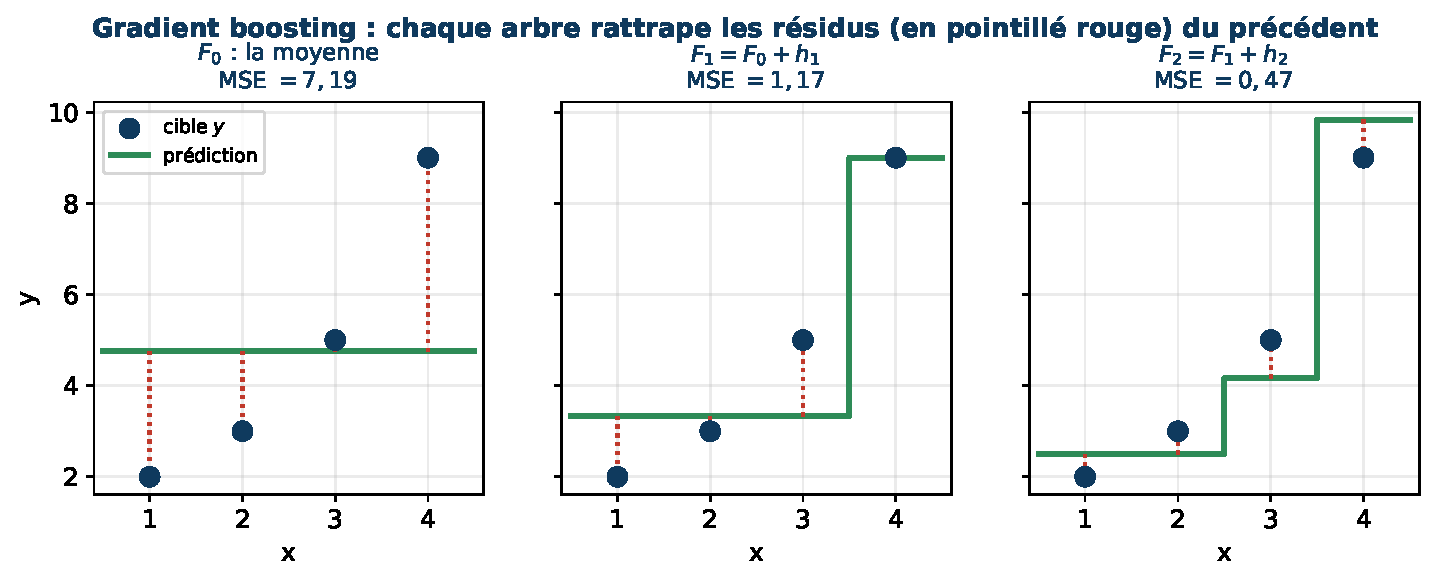
\includegraphics[width=0.90\linewidth]{f8_boosting}
\vspace{-2pt}

{\small Les pointillés rouges — les résidus que chaque arbre doit rattraper — raccourcissent visiblement à chaque étape : la prédiction (en vert) épouse de mieux en mieux la cible. C'est exactement le comportement « apprendre de ses fautes » de l'analogie, rendu quantitatif.}
\end{frame}

\begin{frame}{Pourquoi « gradient » ? le lien avec la Séance 5}
\begin{ucaddef}[Boosting et descente de gradient sont une même idée]
{\small Pour la perte MSE $\tfrac12 (y - F)^2$, la dérivée par rapport à la prédiction $F$ est $-(y - F) = -\,\text{résidu}$. Ajuster un arbre sur les résidus, c'est donc le faire pointer dans la direction $-\nabla(\text{perte})$ : un \emph{pas de descente de gradient}, mais dans l'espace des fonctions au lieu de l'espace des poids.}
\end{ucaddef}
\ucadformula{r_i \;=\; y_i - F(x_i) \;=\; -\,\frac{\partial}{\partial F}\Big[\tfrac12\big(y_i - F(x_i)\big)^2\Big]}
{\small La descente de gradient de la Séance 5 déplaçait des poids $(b, \mathbf{w})$ ; le gradient boosting ajoute des \emph{fonctions} (des arbres), chacune approximant le gradient négatif de la perte. C'est la même mécanique d'optimisation, et c'est pourquoi il fonctionne avec n'importe quelle perte dérivable — dont la log-loss de la Séance 6 pour la classification.}
\end{frame}

\begin{frame}{Le taux d'apprentissage : ne pas tout corriger d'un coup}
\begin{ucaddef}[L'idée en une phrase]
{\small Ajouter chaque arbre \emph{en entier} corrige vite mais brutalement — et finit par rattraper le bruit. On multiplie donc chaque arbre par un petit \textbf{taux d'apprentissage} \texttt{learning\_rate} $\nu$ : des pas plus petits, plus nombreux, plus prudents.}
\end{ucaddef}
\ucadformula{F_{m}(x) \;=\; F_{m-1}(x) \;+\; \nu \cdot h_m(x) \qquad (\nu = \texttt{learning\_rate} \in\, ]0,\ 1])}
{\small C'est le même $\nu$ que le pas de la descente de gradient (Séance 5) : trop grand, on oscille et on rattrape le bruit ; trop petit, on progresse lentement. \texttt{learning\_rate} et \texttt{n\_estimators} se règlent donc \emph{ensemble} — un $\nu$ petit exige plus d'arbres pour le même progrès, mais généralise mieux.}
\end{frame}

\begin{frame}{Le boosting peut sur-apprendre}
\centering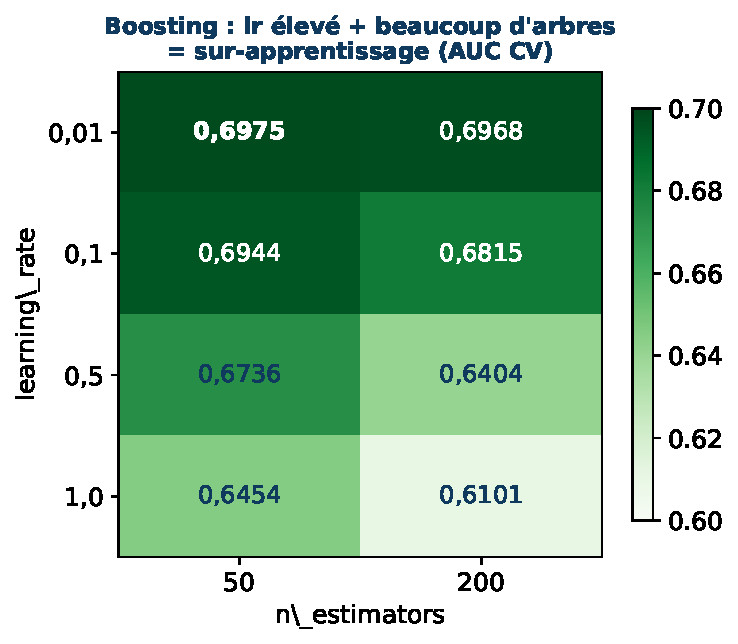
\includegraphics[width=0.44\linewidth]{f8_lr}
\vspace{-2pt}

{\small AUC de validation croisée sur le paludisme, selon le couple $(\nu, \texttt{n\_estimators})$. Le meilleur coin est en haut à gauche — $\nu = 0{,}01$, peu d'arbres : $0{,}698$. En bas à droite — $\nu = 1$, beaucoup d'arbres : $0{,}610$, le modèle a rattrapé le bruit de l'entraînement. \textbf{À l'exact opposé de la forêt} : là où ajouter des arbres faisait plafonner sans risque, ici « plus d'arbres » à grand pas \emph{dégrade}. Le boosting est plus puissant, mais exige le réglage soigneux de la Séance 7.}
\end{frame}

\begin{frame}[fragile]{En pratique : GradientBoostingClassifier}
\begin{lstlisting}
from sklearn.ensemble import GradientBoostingClassifier

gb = GradientBoostingClassifier(n_estimators=100,   # arbres sequentiels
                                learning_rate=0.1,  # pas (a regler avec n_estimators)
                                max_depth=3,         # arbres FAIBLES (peu profonds)
                                random_state=0)
gb.fit(X_train, y_train)
proba = gb.predict_proba(X_test)[:, 1]
\end{lstlisting}
{\small Trois différences de fond avec la forêt : les arbres sont \emph{peu profonds} (des « apprenants faibles » — le biais sera réduit par le \emph{nombre} d'étapes, pas par la profondeur de chacune) ; l'entraînement est \textbf{séquentiel}, donc non parallélisable (chaque arbre attend la prédiction du précédent) ; et le couple \texttt{learning\_rate}/\texttt{n\_estimators} doit être réglé. Les bibliothèques \texttt{XGBoost} et \texttt{LightGBM} en sont des versions optimisées, omniprésentes dans les compétitions et l'industrie.}
\end{frame}

\begin{frame}{Exercice — une étape de boosting à la main}
\begin{ucadrec}[Énoncé]
{\small Sur trois points, la prédiction courante est $F_1 = (3;\ 5;\ 8)$ et la cible $y = (4;\ 4;\ 10)$. (a) Calculer les résidus $r_2 = y - F_1$. (b) Une souche prédit ces résidus par $(+0{,}5;\ +0{,}5;\ +2)$ ; avec $\nu = 0{,}5$, donner la nouvelle prédiction $F_2$. (c) La somme des carrés des résidus a-t-elle diminué ? (d) Un point a-t-il été \emph{sur}-corrigé ?}
\end{ucadrec}
\pause
\begin{ucadex}[Correction]
{\small \textbf{(a)} $r_2 = (4-3;\ 4-5;\ 10-8) = (\mathbf{+1;\ -1;\ +2})$. \textbf{(b)} $F_2 = F_1 + 0{,}5\,(0{,}5;\ 0{,}5;\ 2) = (3{,}25;\ 5{,}25;\ 9{,}00)$. \textbf{(c)} Avant : $1 + 1 + 4 = 6$ ; après : $0{,}5625 + 1{,}5625 + 1 = \mathbf{3{,}125}$ — oui, l'erreur a diminué de moitié. \textbf{(d)} Le point $2$ : son résidu était $-1$, la souche a ajouté $+0{,}25$, l'éloignant légèrement (de $5$ à $5{,}25$, alors que la cible est $4$). Le pas prudent corrige globalement mais peut sur-corriger localement ; d'autres arbres rattraperont.}
\end{ucadex}
\end{frame}

% #####################################################################
\section{Bagging contre boosting}

\begin{frame}{Deux familles, deux mécaniques}
\begin{ucadret}[Le tableau qui tranche]
{\small \begin{center}\renewcommand{\arraystretch}{1.25}
\begin{tabular}{l|l|l}
 & \textbf{forêt aléatoire (bagging)} & \textbf{gradient boosting}\\\hline
arbres & profonds, forts & peu profonds, faibles\\
construits & en \textbf{parallèle} (indépendants) & en \textbf{série} (chacun corrige)\\
agrégation & moyenne / vote ($\div B$) & somme pondérée ($+ \nu h_m$)\\
réduit surtout & la \textbf{variance} & le \textbf{biais}\\
trop d'arbres ? & \textbf{plafonne} (sans risque) & \textbf{sur-apprend} (dérive)\\
réglage clé & \texttt{max\_features} (peu sensible) & $\nu$ et \texttt{n\_estimators} (délicat)\\
parallélisable & oui & non\\
\end{tabular}\end{center}}
\end{ucadret}
\end{frame}

\begin{frame}{Lequel choisir ?}
{\small Une règle de pouce, à nuancer toujours par la validation croisée :}
\begin{itemize}\small
  \item la \textbf{forêt aléatoire} est le \emph{premier réflexe} robuste : peu de réglage, difficile à rater, OOB gratuit, parallélisable — idéale pour un résultat solide rapidement ;
  \item le \textbf{gradient boosting} bien réglé est souvent \emph{plus précis}, surtout quand le signal contient des interactions fines — au prix d'un effort de réglage ($\nu$, \texttt{n\_estimators}) et d'un risque réel de sur-apprentissage ;
  \item dans les deux cas, \textbf{aucune standardisation} n'est nécessaire (ce sont des arbres), et le verdict se prend en validation croisée puis sur le test scellé (Séance 7).
\end{itemize}
{\small Mais « plus précis en général » ne veut pas dire « plus précis ici » : le cas du paludisme va le rappeler avec force.}
\end{frame}

% #####################################################################
\section{Le verdict sur le paludisme}

\begin{frame}{Le grand comparatif}
\centering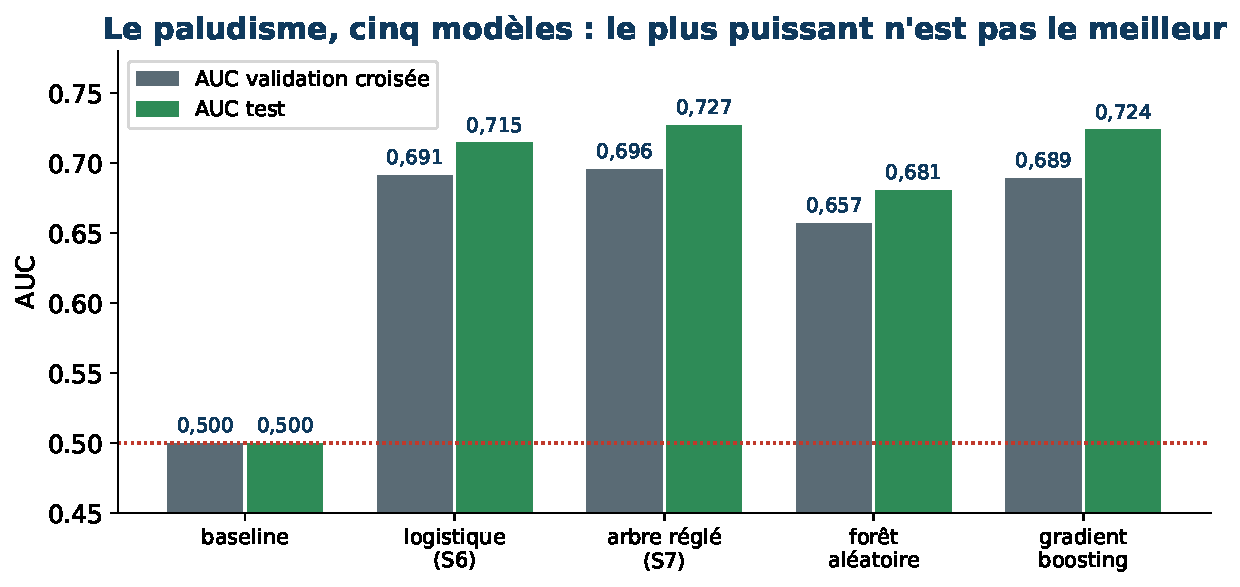
\includegraphics[width=0.64\linewidth]{f8_comparatif}
\vspace{-2pt}

{\small Cinq modèles sur le paludisme, jugés à l'AUC en validation croisée et sur le test (méthode de la Séance 7) : baseline $0{,}50$ ; logistique $0{,}71$ ; arbre réglé $0{,}73$ ; forêt $0{,}68$ ; gradient boosting $0{,}72$. Surprise : les ensembles \emph{ne dominent pas}. L'arbre réglé et la logistique font aussi bien, voire mieux.}
\end{frame}

\begin{frame}{La leçon : plus puissant n'est pas meilleur}
\begin{ucadpiege}[Pourquoi les ensembles ne gagnent pas ici]
{\small Le risque de paludisme, dans ces données, dépend essentiellement de deux variables de façon \emph{simple} (saison, fièvre — c'est ainsi que le jeu est construit). Un modèle linéaire ou un petit arbre capture déjà ce signal. Les forêts et le boosting, en cherchant des interactions complexes dans des variables continues \textbf{non causales} (glycémie, âge), se laissent distraire par le bruit — leur puissance se retourne contre elles.}
\end{ucadpiege}
{\small Ce n'est pas un défaut des ensembles : c'est une \emph{inadéquation} entre la complexité du modèle et celle du problème. La même forêt, sur un jeu riche en interactions, écraserait la logistique.}
\end{frame}

\begin{frame}{Le principe de parcimonie}
\begin{ucaddef}[La morale, généralisée]
{\small \textbf{Aucun modèle n'est supérieur dans l'absolu} (c'est le théorème dit du « no free lunch »). La complexité d'un modèle doit être \emph{justifiée par les données} : on n'emploie une forêt ou un boosting que si le gain en validation croisée le démontre.}
\end{ucaddef}
{\small Conséquence pratique, qui prolonge la discipline de la Séance 7 : comparer honnêtement \emph{tous} les candidats — du plus simple au plus puissant — par validation croisée, puis, \textbf{à performance égale, préférer le plus simple}. Le plus simple est plus rapide à entraîner, plus facile à déployer, plus interprétable, et moins sujet au sur-apprentissage. La puissance ne se paie que lorsqu'elle rapporte.}
\end{frame}

\begin{frame}{Exercice — choisir un modèle}
\begin{ucadrec}[Énoncé]
{\small Sur un problème, on mesure en validation croisée : logistique AUC $0{,}71$, forêt $0{,}72$, gradient boosting réglé $0{,}80$. Sur un \emph{autre} problème : logistique $0{,}90$, forêt $0{,}88$, boosting $0{,}90$. Pour chaque problème, quel modèle retenir, et que peut-on deviner sur la nature du signal ?}
\end{ucadrec}
\pause
\begin{ucadex}[Correction]
{\small \textbf{Problème 1} : le boosting ($0{,}80$) domine nettement — le signal contient probablement des \emph{interactions complexes} que le linéaire et la forêt simple ne captent pas ; la puissance est ici justifiée, on retient le boosting. \textbf{Problème 2} : les trois se valent ($\approx 0{,}90$) — le signal est largement \emph{linéaire}, et l'on choisit la \textbf{logistique} : même performance, modèle plus simple, plus rapide, plus interprétable. À performance égale, la simplicité l'emporte.}
\end{ucadex}
\end{frame}

% #####################################################################
\section{Synthèse}

\begin{frame}{Le protocole d'ensemble}
\begin{ucadret}[De bout en bout]
{\small \textbf{1.} Établir une baseline et un modèle simple (logistique, arbre réglé — Séances 6 et 7) $\to$ \textbf{2.} essayer une \textbf{forêt aléatoire} (quelques centaines d'arbres, défauts) : robuste, peu de réglage, OOB pour un premier diagnostic $\to$ \textbf{3.} si le signal semble riche, essayer un \textbf{gradient boosting} et régler $\nu$/\texttt{n\_estimators} par validation croisée $\to$ \textbf{4.} comparer \emph{tous} les candidats à l'AUC en CV, jamais sur le test $\to$ \textbf{5.} à performance égale, choisir le plus simple $\to$ \textbf{6.} verdict final sur le test scellé, une seule fois.}
\end{ucadret}
\end{frame}

\begin{frame}{À retenir — Séance 8}
\begin{ucadret}[L'essentiel]
\begin{itemize}\small
  \item Agréger des modèles \textbf{décorrélés} bat chacun d'eux — à condition $p > 0{,}5$ \emph{et} erreurs non corrélées (la sagesse de la foule, Condorcet).
  \item La variance d'une moyenne de $B$ arbres tend vers $\rho\,\sigma^2$ : \textbf{décorréler ($\rho \downarrow$), pas seulement multiplier les arbres}.
  \item \textbf{Bagging} : arbres profonds sur des échantillons \emph{bootstrap} ($\approx 63\,\%$ des points), agrégés ; réduit la \textbf{variance} ; l'\textbf{OOB} offre une validation gratuite.
  \item \textbf{Forêt} : bagging $+$ \texttt{max\_features} variables par coupure (décorrélation) ; \texttt{n\_estimators} plafonne (jamais de sur-apprentissage).
  \item L'\textbf{importance des variables} suggère, ne prouve pas — et favorise les variables continues.
  \item \textbf{Boosting} : arbres faibles \emph{séquentiels} rattrapant les résidus ($= -\nabla$ perte) ; réduit le \textbf{biais} ; $\nu \times$ \texttt{n\_estimators} décisif ; \textbf{peut} sur-apprendre.
  \item Leçon centrale : \textbf{le modèle le plus puissant n'est pas toujours le meilleur} — la complexité se justifie par les données (no free lunch).
\end{itemize}
\end{ucadret}
\end{frame}

\begin{frame}{Pièges fréquents (1/2)}
\begin{itemize}\small
  \item Croire qu'un ensemble bat toujours un modèle simple — le comparatif paludisme prouve le contraire.
  \item Penser que multiplier les arbres suffit : sans décorrélation, la variance plafonne à $\rho\,\sigma^2$, élevé.
  \item Régler finement \texttt{n\_estimators} d'une forêt : inutile, ça plafonne — en mettre « assez » suffit.
  \item Lire l'importance des variables comme une preuve de causalité, et oublier son biais vers les variables continues.
\end{itemize}
\end{frame}

\begin{frame}{Pièges fréquents (2/2)}
\begin{itemize}\small
  \item Confondre les deux familles : la forêt réduit la variance (arbres profonds, parallèles), le boosting le biais (arbres faibles, séquentiels).
  \item Pousser \texttt{n\_estimators} d'un boosting à grand \texttt{learning\_rate} : sur-apprentissage garanti.
  \item Standardiser pour une forêt ou un boosting : inutile, les arbres sont insensibles à l'échelle (à la différence de la logistique).
  \item Juger ces modèles sur le test plutôt qu'en validation croisée : la discipline de la Séance 7 reste entière.
\end{itemize}
\end{frame}

\begin{frame}{Prochaine séance}
\begin{ucadfront}[Séance 9 — Apprendre sans étiquettes]
{\small Jusqu'ici, chaque patient portait une étiquette à prédire (durée, paludisme) : c'était l'apprentissage \emph{supervisé}. La Séance 9 lâche les étiquettes : comment \emph{regrouper} des patients similaires sans savoir d'avance en quels groupes — le clustering ($k$-moyennes) — et comment \emph{résumer} des données à beaucoup de variables en en gardant l'essentiel — la réduction de dimension (PCA).}
\end{ucadfront}
\end{frame}

\begin{frame}{Références}
\begin{itemize}\small
  \item James, Witten, Hastie, Tibshirani — \emph{An Introduction to Statistical Learning}, 2\textsuperscript{e} éd., Springer, 2021.
  \item Géron — \emph{Hands-On Machine Learning}, 3\textsuperscript{e} éd., O'Reilly, 2022.
  \item Müller, Guido — \emph{Introduction to Machine Learning with Python}, O'Reilly, 2016.
  \item Hastie, Tibshirani, Friedman — \emph{The Elements of Statistical Learning}, 2\textsuperscript{e} éd., Springer, 2009.
  \item Cours : University of Washington CSE 446 ; Stanford CS229.
\end{itemize}
\end{frame}

\end{document}
